\documentclass[12pt]{report}
\usepackage[margin=1in]{geometry}
\usepackage{setspace} % for single/doublespacing commands
\usepackage{graphicx} % including graphics
\usepackage{sectsty} % sexy section headings
\usepackage[export]{adjustbox} % for graphic frames and center
\usepackage{siunitx}
\usepackage{lmodern} % font package for above
\usepackage[justification=centering]{caption} % figure captions (force centering)
\usepackage{enumitem} % add arguments for enumerate to change style
\usepackage[list=true]{subcaption} % subfigures with list of figure support
\usepackage{multirow}
\usepackage{booktabs}
\usepackage{color}
\usepackage{ulem}
\usepackage[numbers]{natbib}
\usepackage{contour}
\usepackage{tabularx}
\usepackage{framed}
\usepackage{amssymb} % special math symbols
\usepackage{listings}
\usepackage{array}
\usepackage{fancyhdr}
\usepackage{color, colortbl}
\usepackage{tocloft}
\usepackage{url}
\usepackage{etoolbox}
\usepackage{hyperref}
\usepackage{tikz}
\def\checkmark{\tikz\fill[scale=0.4](0,.35) -- (.25,0) -- (1,.7) -- (.25,.15) -- cycle;}
% \setlength{\parskip}{\baselineskip}%
\setlength{\parindent}{0pt}%
\setcounter{secnumdepth}{5}
\renewcommand{\bibname}{References}
\sisetup{output-exponent-marker=\ensuremath{\mathrm{e}}}
\newcommand{\PreserveBackslash}[1]{\let\temp=\\#1\let\\=\temp}
\newcolumntype{C}[1]{>{\PreserveBackslash\centering}p{#1}}
\newcolumntype{R}[1]{>{\PreserveBackslash\raggedleft}p{#1}}
\newcolumntype{L}[1]{>{\PreserveBackslash\raggedright}p{#1}}
\lstMakeShortInline[style=Matlab-editor]| % matlab inline escape character
\graphicspath{{images/}}
\renewcommand\thesection{\arabic{section}}
\renewcommand\labelitemi{---}
\lstset{numberstyle=\ttfamily\small\color{gray}}

\apptocmd{\sloppy}{\hbadness 10000\relax}{}{}
\setlength{\cftbeforetoctitleskip}{-2em}
\allsectionsfont{\raggedright}
\setlist[enumerate]{wide=0pt, widest=99,
                    leftmargin=\parindent,topsep=0pt,partopsep=0pt,
                    label=\thesubsubsection.\alph*,font=\itshape}



\begin{document}
\normalem
\begin{titlepage}
\flushleft
\doublespacing
\Large
\textsc{Test Document} \\
\normalsize
Trey Dufrene, Zack Johnson, David Orcutt, Alan Wallingford, Ryan Warner
\vfill
\center
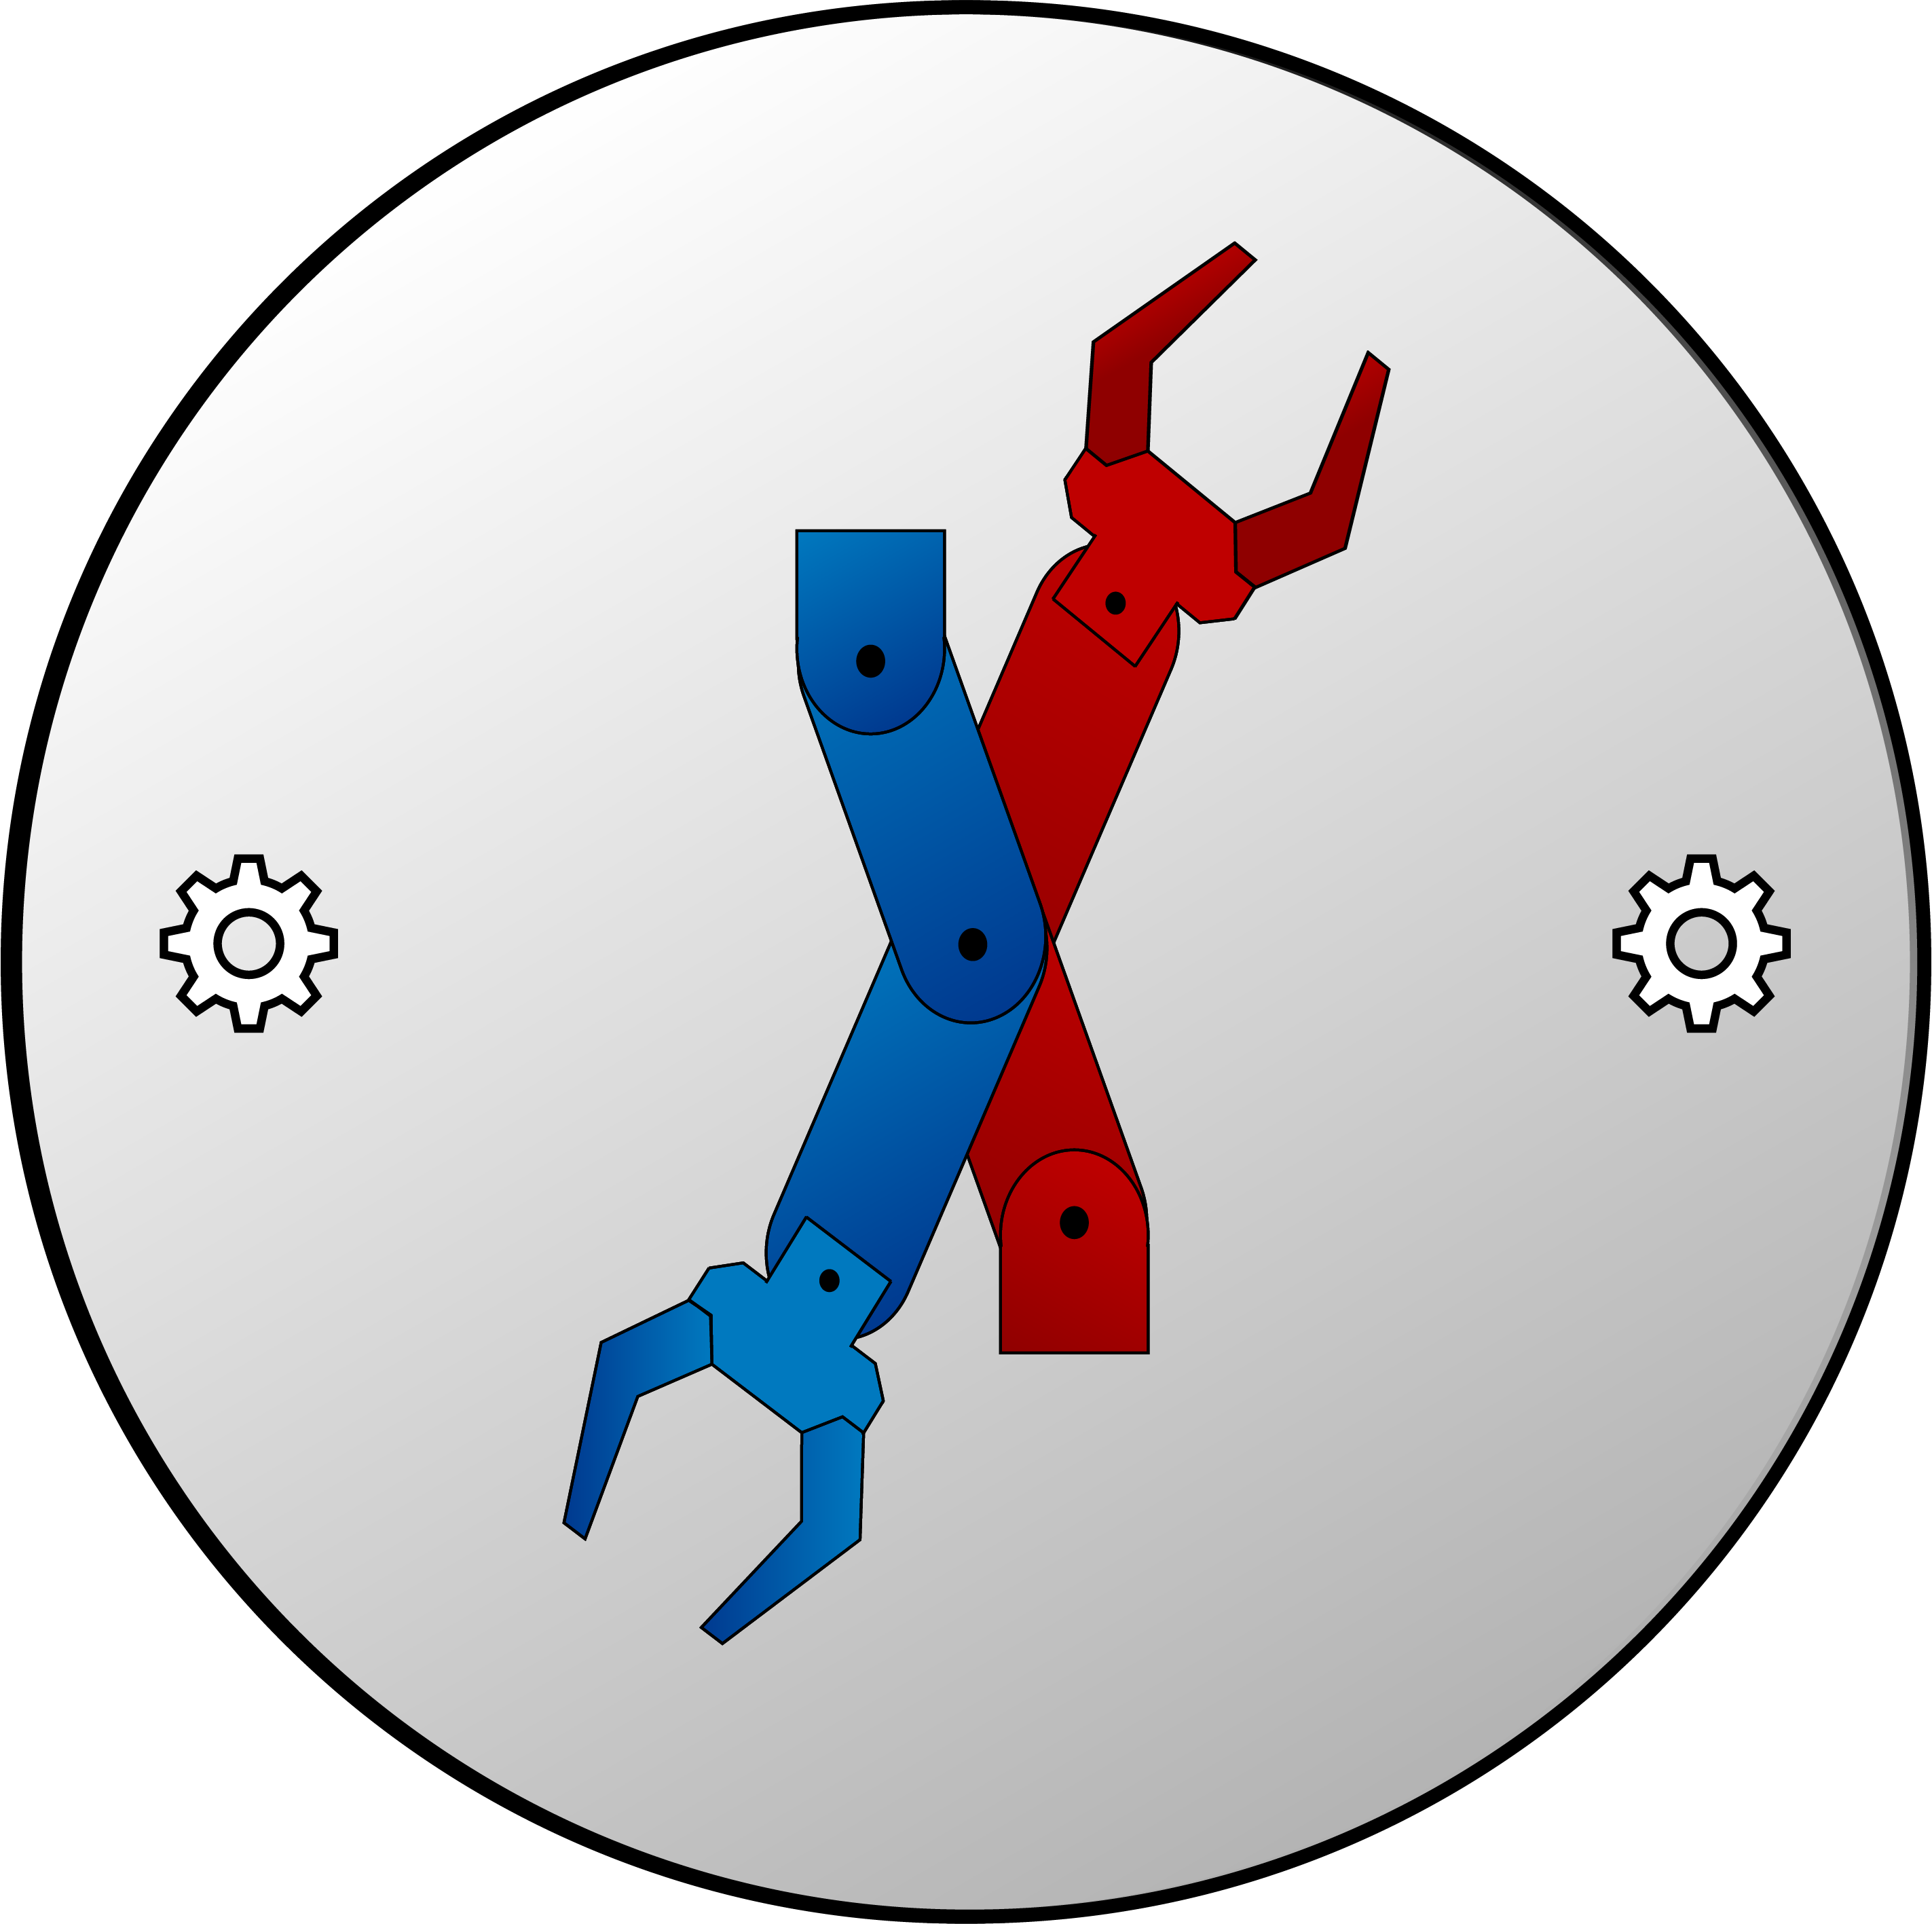
\includegraphics[width=.45\textwidth]{logo}
\vfill
\flushleft
ME 407 \\
Preliminary Design of Robotic Systems \\
Embry-Riddle Aeronautical University \\
\vspace{2ex}
\begin{minipage}[c]{.5\textwidth}
\flushleft

\includegraphics[width=.95\textwidth]{erau}
\end{minipage}%
\begin{minipage}[c]{.5\textwidth}
\flushright

\includegraphics[width=.8\textwidth]{text}
\end{minipage}
\end{titlepage}

\pagenumbering{roman}
% \begin{abstract}
  % Wordy words
% \end{abstract}
{\tableofcontents\let\clearpage\relax\listoffigures}
\clearpage
\newpage
\pagenumbering{arabic}

\section{Introduction}\label{sec:intro}
\raggedright
\section{Specifications and Tests}
\section{Conclusion}

\begin{table}[htp]
  \centering
  \caption{Summary of Test Results}
  \label{tab:results}
  \begin{tabular}{c|c}
  Specification Tested & Specification Met? \\ \hline
  1.1.a & \\
  1.2.a & \checkmark \\
  1.2.b & \checkmark \\
  1.3.a & Cannot be Determined \\
  1.4.a & Cannot be Determined \\
  1.4.b & Cannot be Determined \\
  1.4.c & Cannot be Determined \\
  1.5.a & \checkmark \\
  1.5.b & \checkmark \\
  1.6.a & \checkmark \\
  1.6.b & $\times$ \\
  1.7.a & \checkmark \\
  1.7.b & Cannot be Determined \\
  1.8.a & Cannot be Determined \\
  2.1.a & \\
  2.2.a & \\
  2.2.b & \checkmark \\
  \end{tabular}
\end{table}
\newpage
\appendix
\renewcommand\thesection{\Roman{section}}
\renewcommand\thesubsection{\roman{subsection}}
\section*{Appendix}\label{sec:app}


\newpage
\bibliographystyle{plainnat}
\bibliography{robo}


\end{document}
